\subsection{D-Latch} % (fold)
\label{sub:D-Latch}
\begin{frame}
    \frametitle{D-Latch}
    \framesubtitle{}
    \begin{figure}[H]
    \begin{center}
            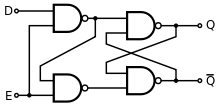
\includegraphics[scale=0.6]{./img/schaltung/D-Latch.png}
    \end{center}
    \end{figure}
\end{frame}
\begin{frame}
    \frametitle{Funktionsweise}
    \framesubtitle{}
    \begin{columns}[c]
        \column{0.6\textwidth}
            bla 
        \column{0.4\textwidth}
            \begin{figure}[H]
            \begin{center}
                    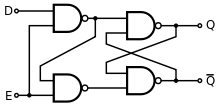
\includegraphics[scale=0.6]{./img/schaltung/D-Latch.png}
            \end{center}
            \end{figure}
            \begin{figure}[H]
            \begin{center}
                    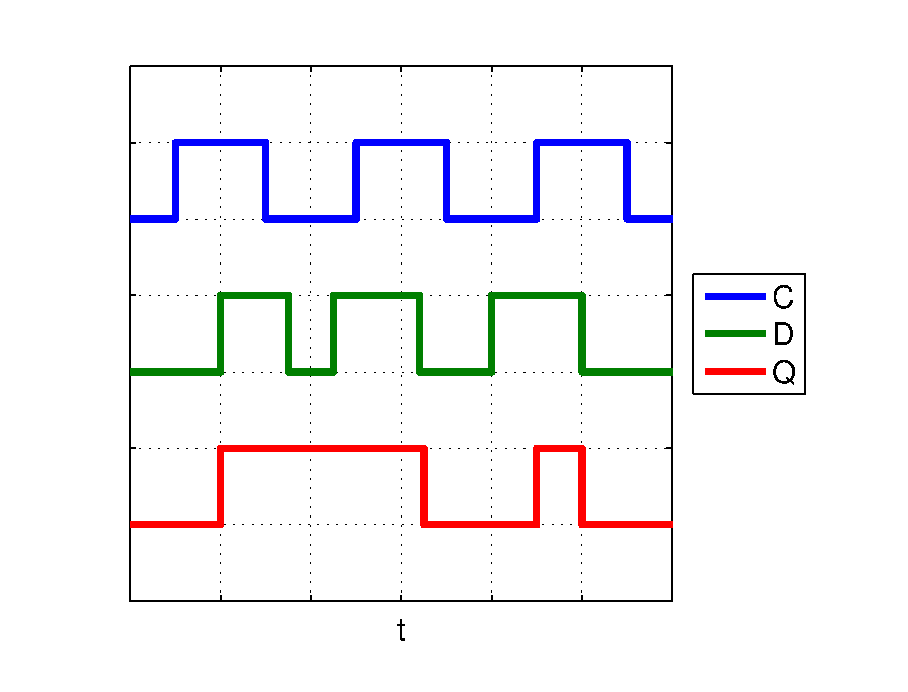
\includegraphics[scale=0.3]{./img/Aufgabe_2_c.eps}
            \end{center}
            \end{figure}
    \end{columns}
\end{frame}
% subsection D-Latch (end)
